%!TEX root = ../report.tex

\chapter{Evaluation and Results}

Both the Mohler datasets were used in our experiments of grading with Active Learning and accuracy was used as an evaluation metric. 

\section{Experiment 1}

The tasks carried out could be categorized into two parts, namely, binary classification (where the grader predicts whether the answers are correct or wrong) and multi-class classification (where the grader predicts a whole number grade for each answer after being trained from the rounded off answer-grade pairs).

\subsection{Binary Classification}

The grades of the answers which are below 3 were considered as wrong answers and the others were considered as correct answers. The task includes training the initial model (Logistic Regression Classifier in our experiment) with one answer-grade pair for each class (correct and incorrect) and then 40 answers were queried from a human for the correct grade. These answers which were queried from the human was selected based on the Active Learning strategy called uncertainty-based sampling. 

A comparison was made between this strategy and Supervised Learning. As can been seen in Fig. \ref{m1_binary}, active learning was able to achieve an accuracy of 88.14\% while supervised learning was able to reach only 82.23\%.

\begin{figure}[h!]
	\centering
	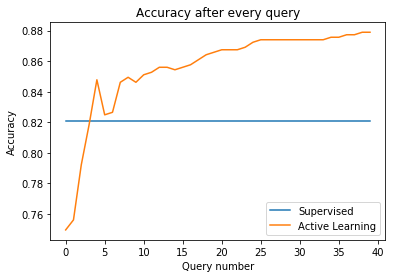
\includegraphics[scale=0.7]{images/m1_binary}
	\caption{Comparison in terms of accuracy between active learning and supervised learning in the Mohler 2009 dataset.}
	\label{m1_binary}
\end{figure}

Similar task was carried out on the Mohler 2011 dataset. As can been seen in Fig. \ref{m2_binary}, active learning was able to achieve an accuracy of 87.31\% while supervised learning was able to reach only 87.73\%. It could be inferred that with proper features and more queries, active learning could perform better than supervised learning.

\begin{figure}[h!]
	\centering
	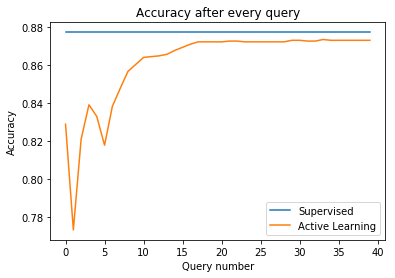
\includegraphics[scale=0.7]{images/m2_binary}
	\caption{Comparison in terms of accuracy between active learning and supervised learning in the Mohler 2011 dataset.}
	\label{m2_binary}
\end{figure}


\subsection{Multi-class Classification}

The grades were rounded off to the nearest whole number (which ended up in six classes in the range of 0 to 5). The task includes training the initial model (Logistic Regression Classifier in our experiment) with one answer-grade pair for each of class  and then 40 answers were queried from a human for the correct grade. These answers which were queried from the human was selected based on the Active Learning strategy called uncertainty-based sampling. 

A comparison was made between this strategy and Supervised Learning on the Mohler 2009 dataset. As can been seen in Fig. \ref{m1_multi}, active learning was able to achieve an accuracy of 52.21\% while supervised learning was able to reach only 61.78\%.

\begin{figure}[h]
	\centering
	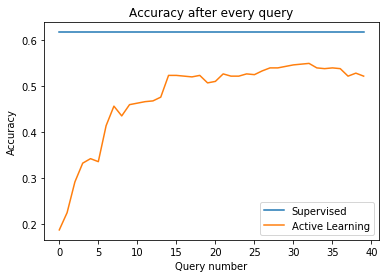
\includegraphics[scale=0.7]{images/m1_multi}
	\caption{Comparision in terms of accuracy between active learning and supervised learning in the Mohler 2009 dataset.}
	\label{m1_multi}
\end{figure}

Similar task was carried out on the Mohler 2011 dataset. As can been seen in Fig. \ref{m2_multi}, active learning was able to achieve an accuracy of 48.44\% while supervised learning was able to reach only 59.71\%. It could be inferred that with proper features and more queries, active learning could perform better than supervised learning in the multi-class classification. \\

\begin{figure}[h!]
	\centering
	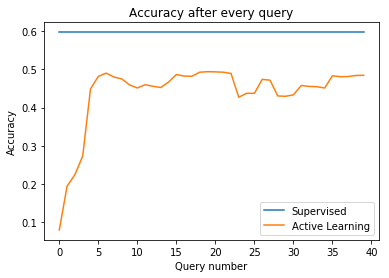
\includegraphics[scale=0.7]{images/m2_multi}
	\caption{Comparison in terms of accuracy between active learning and supervised learning in the Mohler 2011 dataset.}
	\label{m2_multi}
\end{figure}


The results have been tabulated in the table \ref{results} below.\\ 

\begin{table}[]
\centering
\begin{tabular}{|c|c|c|c|}
\hline
                                                                                 &                            & \textbf{\begin{tabular}[c]{@{}c@{}}Active \\ Learning\end{tabular}} & \textbf{\begin{tabular}[c]{@{}c@{}}Supervised\\ Learning\end{tabular}} \\ \hline
\multirow{2}{*}{\textbf{\begin{tabular}[c]{@{}c@{}}Mohler \\ 2009\end{tabular}}} & Binary classification      & \textbf{88.14\%}                                                    & 82.23\%                                                                \\ \cline{2-4} 
                                                                                 & Multi-class classification & 52.21\%                                                             & \textbf{61.78\%}                                                       \\ \hline
\multirow{2}{*}{\textbf{\begin{tabular}[c]{@{}c@{}}Mohler \\ 2011\end{tabular}}} & Binary classification      & 83.31\%                                                             & \textbf{83.73\%}                                                       \\ \cline{2-4} 
                                                                                 & Multi-class classification & 48.44\%                                                             & \textbf{59.71\%}                                                       \\ \hline
\end{tabular}
\caption{Experiment results on both Mohler 2009 and Mohler 2011 dataset.}
\label{results}
\end{table}

\section{Experiment 2}

As discussed in the Experimental Setup section above, users were asked to test the system with and without the help of active learning. A questionaire was prepared to get feedbacks from them about their experience which is given below. 

\newpage
\subsection{User 1}

Total clicks taken without active learning - 90 clicks \\
Total clicks taken with active learning - 52 clicks
\begin{itemize}
\item How easy is our grading to use ? \\
In a scale of 1-10 , I would rate it as 6. 
\item Did AI assisted grading reduce the effort of grading ? \\
Yes. The difference was very clear. In manual grading I need to select the grades for all the answers and have to submit the grade. While in case of AI assisted grading most of the times I just need to verify the graded answer. Hence lots of effort for grading is reduced.
\item How about the readability of Questions and answers ? \\
The readability of question and answers was fine. Still, Various fonts can be tried to help the user find the better font for reading.
\item How about the positioning and sizing of various elements (radio button,submit button)? \\
Size of the radio button can be increased. Submit button can be on the right side as most of the users are right handed. 
\item What features you think need to be added to enhance the experience ? \\
Same question with different student answers can be displayed in a single page.
\end{itemize}

\subsection{User 2}

Total clicks taken without active learning - 90 clicks \\
Total clicks taken with active learning - 56 clicks
\begin{itemize}

\item How easy is our grading to use ? \\
In a scale of 1-10 , I would rate it as 7. 
\item Did AI assisted grading reduce the effort of grading ? \\
Yes. 
\item How about the readability of Questions and answers ? \\
Readability was satisfactory.
\item How about the positioning and sizing of various elements (radio button,submit button)? \\
Positioning can be improved a bit as I have to move the cursor here and there for selection. Instead it would be great if the movement of the cursor was in a sequential manner.
\item What you think need to be added to enhance the experience ? \\
Lot can be added to make the user feel comfortable. Various display options can be created. Autograding score can be embedded in other options other than radio button. Shortcuts can be created.
\end{itemize}
